%
% trafo.tex
%
% (c) 2019 Prof Dr Andreas Müller, Hochschule Rapperswil
%

\def\curve#1#2#3{
\begin{scope}
\clip (-6.5,-3) rectangle (6.5,3);
\draw[line width=1pt,color=red]
	plot[domain={((#2)-2*abs(#1))}:{((#2)+2*abs(#1))},samples=100]
	({\x},{(#3)*sin(8*((\x-(#2))/(#1))*(180/3.1415))*exp(-((\x-(#2))/(#1))*((\x-(#2))/(#1)))/sqrt(abs(#1))});
\end{scope}
}

\def\flaeche#1#2#3{
\begin{scope}
\clip (-6.5,-3) rectangle (6.5,3);
\fill[color=red!20]
	plot[domain={((#2)-2*abs(#1))}:{((#2)+2*abs(#1))},samples=200]
	({\x},{(#3)*exp(-((\x-(#2))/(#1))*((\x-(#2))/(#1)))/sqrt(abs(#1))})
	--
	plot[domain={((#2)+2*abs(#1))}:{((#2)-2*abs(#1))},samples=200]
	({\x},{-(#3)*exp(-((\x-(#2))/(#1))*((\x-(#2))/(#1)))/sqrt(abs(#1))})
	--cycle;
\end{scope}
}

\def\achsen#1{
	\draw[->,line width=0.7pt] (-6.6,0)--(7.0,0) coordinate[label={$t$}];
	\draw[->,line width=0.7pt] (0,{-#1})--(0,{#1});
	\foreach \x in {1,...,6}{
		\draw[line width=0.7pt] ({\x},-0.08)--({\x},0.08);
		\draw[line width=0.7pt] ({-\x},-0.08)--({-\x},0.08);
	}
}

\def\cwt#1#2#3{
	\draw[->,line width=0.7pt]
		(-6.6,{#3-2})--(7.0,{#3-2}) coordinate[label={$b$}];
	\draw[->,line width=0.7pt]
		(0,{#3-2.1})--(0,{#3+0.4}) coordinate[label={left:$a$}];
	\fill[color=red] ({#2},{#3-2+#1}) circle[radius=0.08];
}

%\documentclass[tikz]{standalone}
\usepackage{amsmath}
\usepackage{pgfplots}
\usepackage{csvsimple}

\usetikzlibrary{arrows,intersections,math}

\begin{document}
\begin{tikzpicture}[>=latex,scale=0.95]

\begin{axis}[width=15cm, height=7.5cm, xmin=-4, xmax=4, ymin=-1.2, ymax=1.2,
		axis lines=middle, ytick={-1, -0.5, ..., 1}, xtick={-3, -2, ..., 3}]
	\addplot[smooth, mark=none, color=blue] table[x=t,y=h] {gabor.data};
	\addplot[fill=gray, opacity=0.1]  table[x=t,y=envp] {gabor.data};
	\addplot[fill=gray, opacity=0.1]  table[x=t,y=envn] {gabor.data};
\end{axis}

\end{tikzpicture}
\end{document}


%%
% translation.tex
%
% (c) 2019 Prof Dr Andreas Müller, Hochschule Rapperswil
%
\begin{frame}
\frametitle{Translation}

\begin{center}
\begin{tikzpicture}[>=latex]

\draw[line width=1pt,color=blue!40] (-6.5,-3)--(6.5,-3);

\ifthenelse{\boolean{presentation}}{
\node at (0,2) [left] {$T_{b}\psi(t)=\mathstrut$};


\foreach \b in {1,...,10}{
	\only<\b>{
		\pgfmathparse{0.5*(\b-11)}
		\xdef\B{\pgfmathresult}
		\pgfmathparse{-\B}
		\xdef\minusB{\pgfmathresult}
		\node at (0,2) [right] {$T_{\B}\psi(t)=\psi(t+\minusB)$};
		\flaeche{1}{\B}{1}
		\achsen{1.5}
		\curve{1}{\B}{1}
		\cwt{1}{\B}{-2.0}
	}
}
\only<11>{
	\node at (0,2) [right] {$T_0\psi(t)=\psi(t)$};
	\flaeche{1}{0}{1}
	\achsen{1.5}
	\curve{1}{0}{1}
	\cwt{1}{0}{-2.0}
}
\foreach \b in {12,...,21}{
	\only<\b>{
		\pgfmathparse{0.5*(\b-11)}
		\xdef\B{\pgfmathresult}
		\pgfmathparse{-\B}
		\xdef\minusB{\pgfmathresult}
		\node at (0,2) [right] {$T_{\B}\psi(t)=\psi(t-\B)$};
		\flaeche{1}{\B}{1}
		\achsen{1.5}
		\curve{1}{\B}{1}
		\cwt{1}{\B}{-2.0}
	}
}
}{
	\node at (0,2) {$T_{b}\psi(t)= T_{3}\psi(t)=\psi(t-3)$};
	\flaeche{1}{3}{1}
	\achsen{1.5}
	\curve{1}{3}{1}
	\cwt{1}{3}{-2.0}
}

\end{tikzpicture}
\end{center}

\end{frame}



%%
% dilatation.tex -- template for standalon tikz images
%
% (c) 2019 Prof Dr Andreas Müller, Hochschule Rapperswil
%
\documentclass[tikz]{standalone}
\usepackage{amsmath}
\usepackage{times}
\usepackage{txfonts}
\usepackage{pgfplots}
\usepackage{csvsimple}
\usetikzlibrary{arrows,intersections,math}
\begin{document}
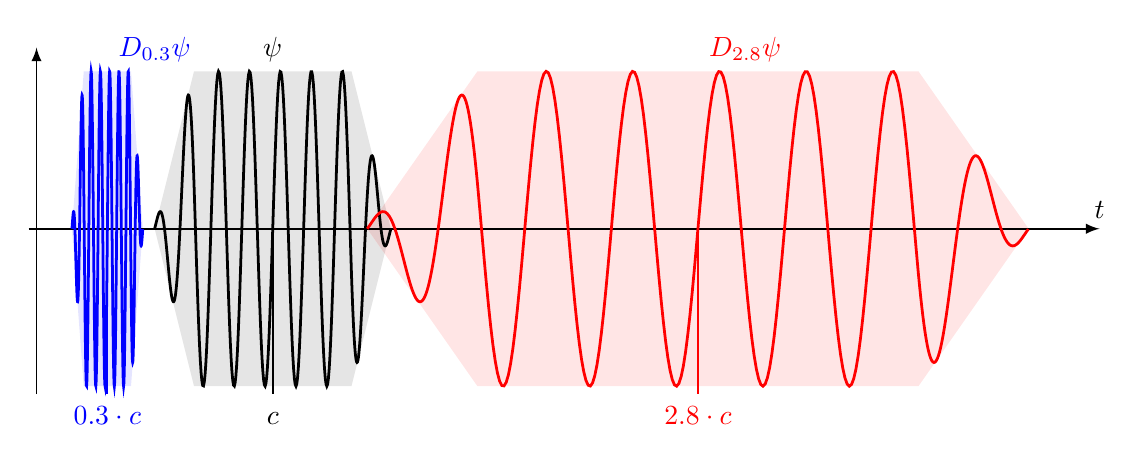
\begin{tikzpicture}[>=latex]

\def\pivalue{3.14159}

\def\bone{2.8}
\def\btwo{0.3}
\def\frequency{16}

\fill[color=gray!20] (1.5,0)--(2,-2)--(4,-2)
	--(4.5,0)--(4,2)--(2,2)--cycle;

\fill[color=blue!10] ({1.5*\btwo},0)--({2*\btwo},-2)--({4*\btwo},-2)
	--({4.5*\btwo},0)--({4*\btwo},2)--({2*\btwo},2)--cycle;
\fill[color=red!10] ({1.5*\bone},0)--({2*\bone},-2)--({4*\bone},-2)
	--({4.5*\bone},0)--({4*\bone},2)--({2*\bone},2)--cycle;

\begin{scope}
\clip (1.5,0)--(2,-2)--(4,-2)--(4.5,0)--(4,2)--(2,2)--cycle;
\definecolor{bluegray}{rgb}{0.8,0.8,0.9}
\definecolor{redgray}{rgb}{0.9,0.8,0.8}
\fill[color=bluegray] ({1.5*\btwo},0)--({2*\btwo},-2)--({4*\btwo},-2)
	--({4.5*\btwo},0)--({4*\btwo},2)--({2*\btwo},2)--cycle;
\fill[color=redgray] ({1.5*\bone},0)--({2*\bone},-2)--({4*\bone},-2)
	--({4.5*\bone},0)--({4*\bone},2)--({2*\bone},2)--cycle;
\end{scope}

\draw[->,line width=0.7pt] (-0.1,0)--(13.5,0) coordinate[label={$t$}];
\draw[->,line width=0.7pt] (0,-2.1)--(0,2.3);

%\foreach \x in {1,...,13}{
%	\draw[line width=0.7pt] ({\x},-0.1)--({\x},0.1);
%}

\node at (3,2) [above] {$\psi$};
\node[color=blue] at (1.5,2) [above] {$D_{\btwo}\psi$};
\node[color=red] at (9,2) [above] {$D_{\bone}\psi$};

\draw[line width=1pt]
	plot[domain=-1.5:-1,samples=100]
		({\x+3},{2*2*(\x+1.5)*sin(\frequency*\x*(180/\pivalue))}) --
	plot[domain=-1:1,samples=200]
		({\x+3},{2*sin(\frequency*\x*(180/\pivalue))}) --
	plot[domain=1:1.5,samples=100]
		({\x+3},{-2*2*(\x-1.5)*sin(\frequency*\x*(180/\pivalue))});

\draw[color=blue,line width=1pt]
	plot[domain=-1.5:-1,samples=100]
		({(\x+3)*\btwo},{2*2*(\x+1.5)*sin(\frequency*\x*(180/\pivalue))}) --
	plot[domain=-1:1,samples=200]
		({(\x+3)*\btwo},{2*sin(\frequency*\x*(180/\pivalue))}) --
	plot[domain=1:1.5,samples=100]
		({(\x+3)*\btwo},{-2*2*(\x-1.5)*sin(\frequency*\x*(180/\pivalue))});

\draw[color=red,line width=1pt]
	plot[domain=-1.5:-1,samples=100]
		({(\x+3)*\bone},{2*2*(\x+1.5)*sin(\frequency*\x*(180/\pivalue))}) --
	plot[domain=-1:1,samples=200]
		({(\x+3)*\bone},{2*sin(\frequency*\x*(180/\pivalue))}) --
	plot[domain=1:1.5,samples=100]
		({(\x+3)*\bone},{-2*2*(\x-1.5)*sin(\frequency*\x*(180/\pivalue))});

\draw[color=red,line width=0.7pt] ({3*\bone},0)--({3*\bone},-2.1);
\node[color=red] at ({3*\bone},-2.1) [below] {$\bone\cdot c\mathstrut$};
\draw[color=blue,line width=0.7pt] ({3*\btwo},0)--({3*\btwo},-2.1);
\node[color=blue] at ({3*\btwo},-2.1) [below] {$\btwo\cdot c\mathstrut$};
\draw[line width=0.7pt] (3,0)--(3,-2.1);
\node at (3,-2.1) [below] {$c\mathstrut$};

\end{tikzpicture}
\end{document}



%
% transdil.tex
%
% (c) 2019 Prof Dr Andreas Müller, Hochschule Rapperswil
%
\ifthenelse{\boolean{presentation}}{

\begin{frame}
\frametitle{Translation und Dilation}
\begin{center}
\begin{tikzpicture}[>=latex]

\draw[color=blue!40,line width=1pt] plot[domain=-6:6,samples=100]
	({\x},{1.1+cos(\x*(180/3.1415))-4});

\def\bmax{101}
\pgfmathparse{0.5*(\bmax-1)}
\xdef\s{\pgfmathresult}

\foreach \b in {1,...,{\bmax}}{
	\only<\b>{
		\pgfmathparse{6*((\b)-1-\s)/(\s)}
		\xdef\B{\pgfmathresult}
		\pgfmathparse{1.1+cos(\B*180/3.1415)}
		\xdef\A{\pgfmathresult}
		\flaeche{\A}{\B}{1}
		\achsen{1.5}
		\curve{\A}{\B}{1}
		\cwt{\A}{\B}{-2.0}
	}
}

\end{tikzpicture}
\end{center}
\end{frame}

}{}








